\input{../YKY-preamble.tex}

\usepackage{color}
\usepackage{mathtools}
\usepackage{hyperref}

% \usepackage[backend=biber,style=numeric]{biblatex}
% \bibliography{../AGI-book}
% \renewcommand*{\bibfont}{\footnotesize}

\usepackage{graphicx} % Allows including images
\usepackage{tikz-cd}
\usepackage{tikz}
\usetikzlibrary{shapes}
\usepackage[export]{adjustbox}% http://ctan.org/pkg/adjustbox
\usepackage{bm}
\usepackage{verbatim} % for comments
\usepackage[most]{tcolorbox}
% \usepackage{newtxtext,newtxmath}	% Times New Roman font

\setcounter{secnumdepth}{1}		% no sub-section numbers
% \numberwithin{equation}{subsection}

\newcommand{\underdash}[1]{%
	\tikz[baseline=(toUnderline.base)]{
		\node[inner sep=1pt,outer sep=10pt] (toUnderline) {#1};
		\draw[dashed] ([yshift=-0pt]toUnderline.south west) -- ([yshift=-0pt]toUnderline.south east);
	}%
}%

\newcommand{\bO}[0]{$\pmb{\bm{\Circle}}$}
\newcommand{\bX}[0]{$\pmb{\bm{\times}}$}

\DeclareSymbolFont{symbolsC}{U}{txsyc}{m}{n}
\DeclareMathSymbol{\strictif}{\mathrel}{symbolsC}{74}

\newcommand{\highlight}[1]{\colorbox{pink}{$\displaystyle #1$}}

\newcommand{\emp}[1]{{\color{violet}\textbf{#1}}}
\newcommand*\confoundFace{$\vcenter{\hbox{\includegraphics[scale=0.2]{../2020/../confounded-face.jpg}}}$}
\newcommand{\underconst}{\includegraphics[scale=0.5]{../2020/UnderConst.png}}
\newcommand{\witness}{\scalebox{0.6}{$\blacksquare$}}
% \newcommand{\Heytingarrow}{\mathrel{-}\mathrel{\triangleright}}
\providecommand\Heytingarrow{\relbar\joinrel\mathrel{\vcenter{\hbox{\scalebox{0.75}{$\rhd$}}}}}
\renewcommand*\sigmoid{\vcenter{\hbox{\includegraphics[scale=2.0]{../sigmoid3.png}}}}

\newcommand{\bbb}[1]{\tcbox[size=small, box align=base,nobeforeafter]{#1}} 

\begin{document}

\title{\bfseries\color{blue}{\Huge AGI for dummies: 1}}
\author{YKY} % Your name
%\institute[] % Your institution as it will appear on the bottom of every slide, may be shorthand to save space
%{
%Independent researcher, Hong Kong \\ % Your institution for the title page
%\medskip
%\textit{generic.intelligence@gmail.com} % Your email address
%}
\date{\today} % Date, can be changed to a custom date

\maketitle

% \vspace*{0.5cm}
% 多谢 支持 \smiley

% \setcounter{section}{-1}
\subsection{The biological neuron}

Electrical signals are collected by dendrites where they are \textbf{summed up} around the cell body.  If the sum total of electrical signals is greater than a certain fixed \textbf{threshold}, the neuron fires a new electric impulse at its output:
\begin{equation}
\vcenter{\hbox{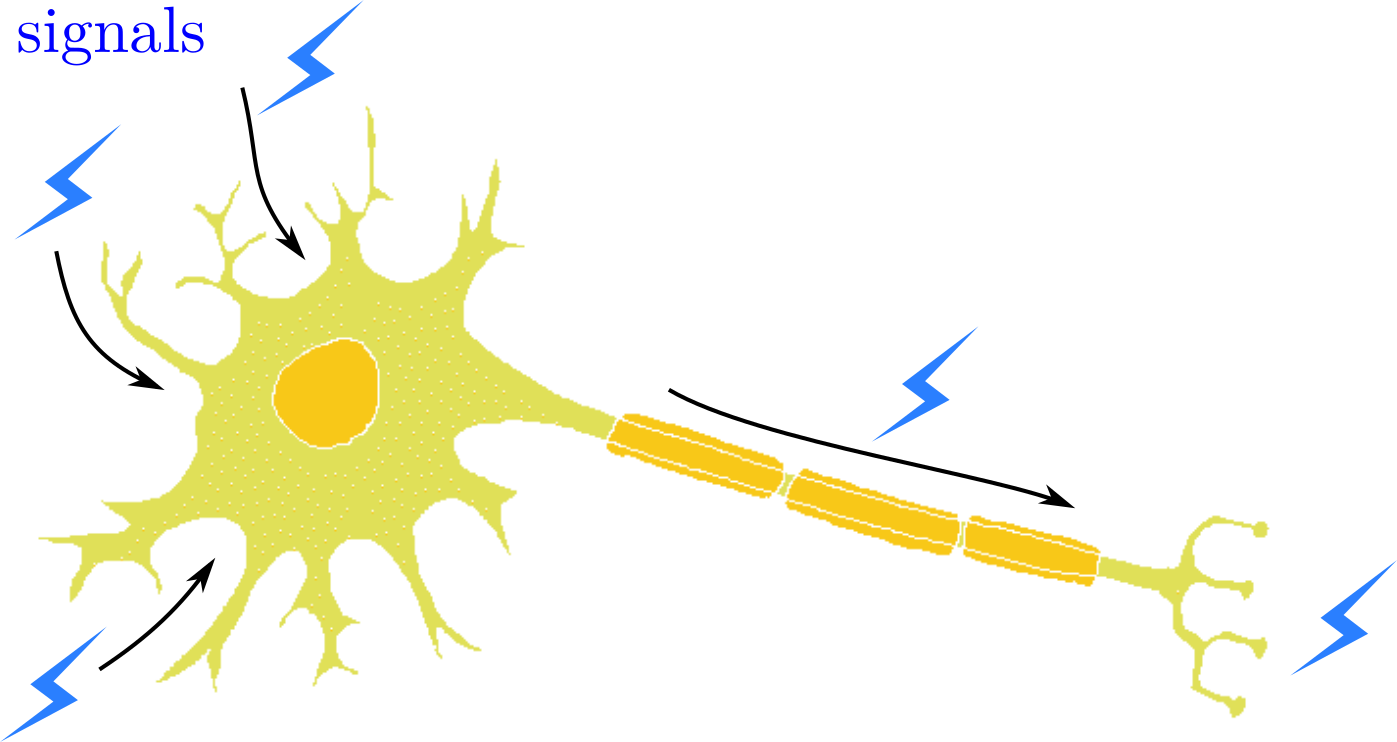
\includegraphics[scale=0.7]{biological-neuron-dummies.png}}}
\end{equation}

Human cells are very simple ``machines''.  They cannot perform highly complex computations.  Each neuron performs only this simple operation, and together they achieve the powerful cognitive abilities of the brain.

\subsection{The mathematical neuron}

Mathematically, a neuron is represented by this formula:
\begin{equation}
\boxed{\mbox{output}} \quad y = \sigmoid \left( \; \sum W \cdot x \right) \quad \boxed{\mbox{input}}
\end{equation}


\subsection{The neural network}

\begin{equation}
\vcenter{\hbox{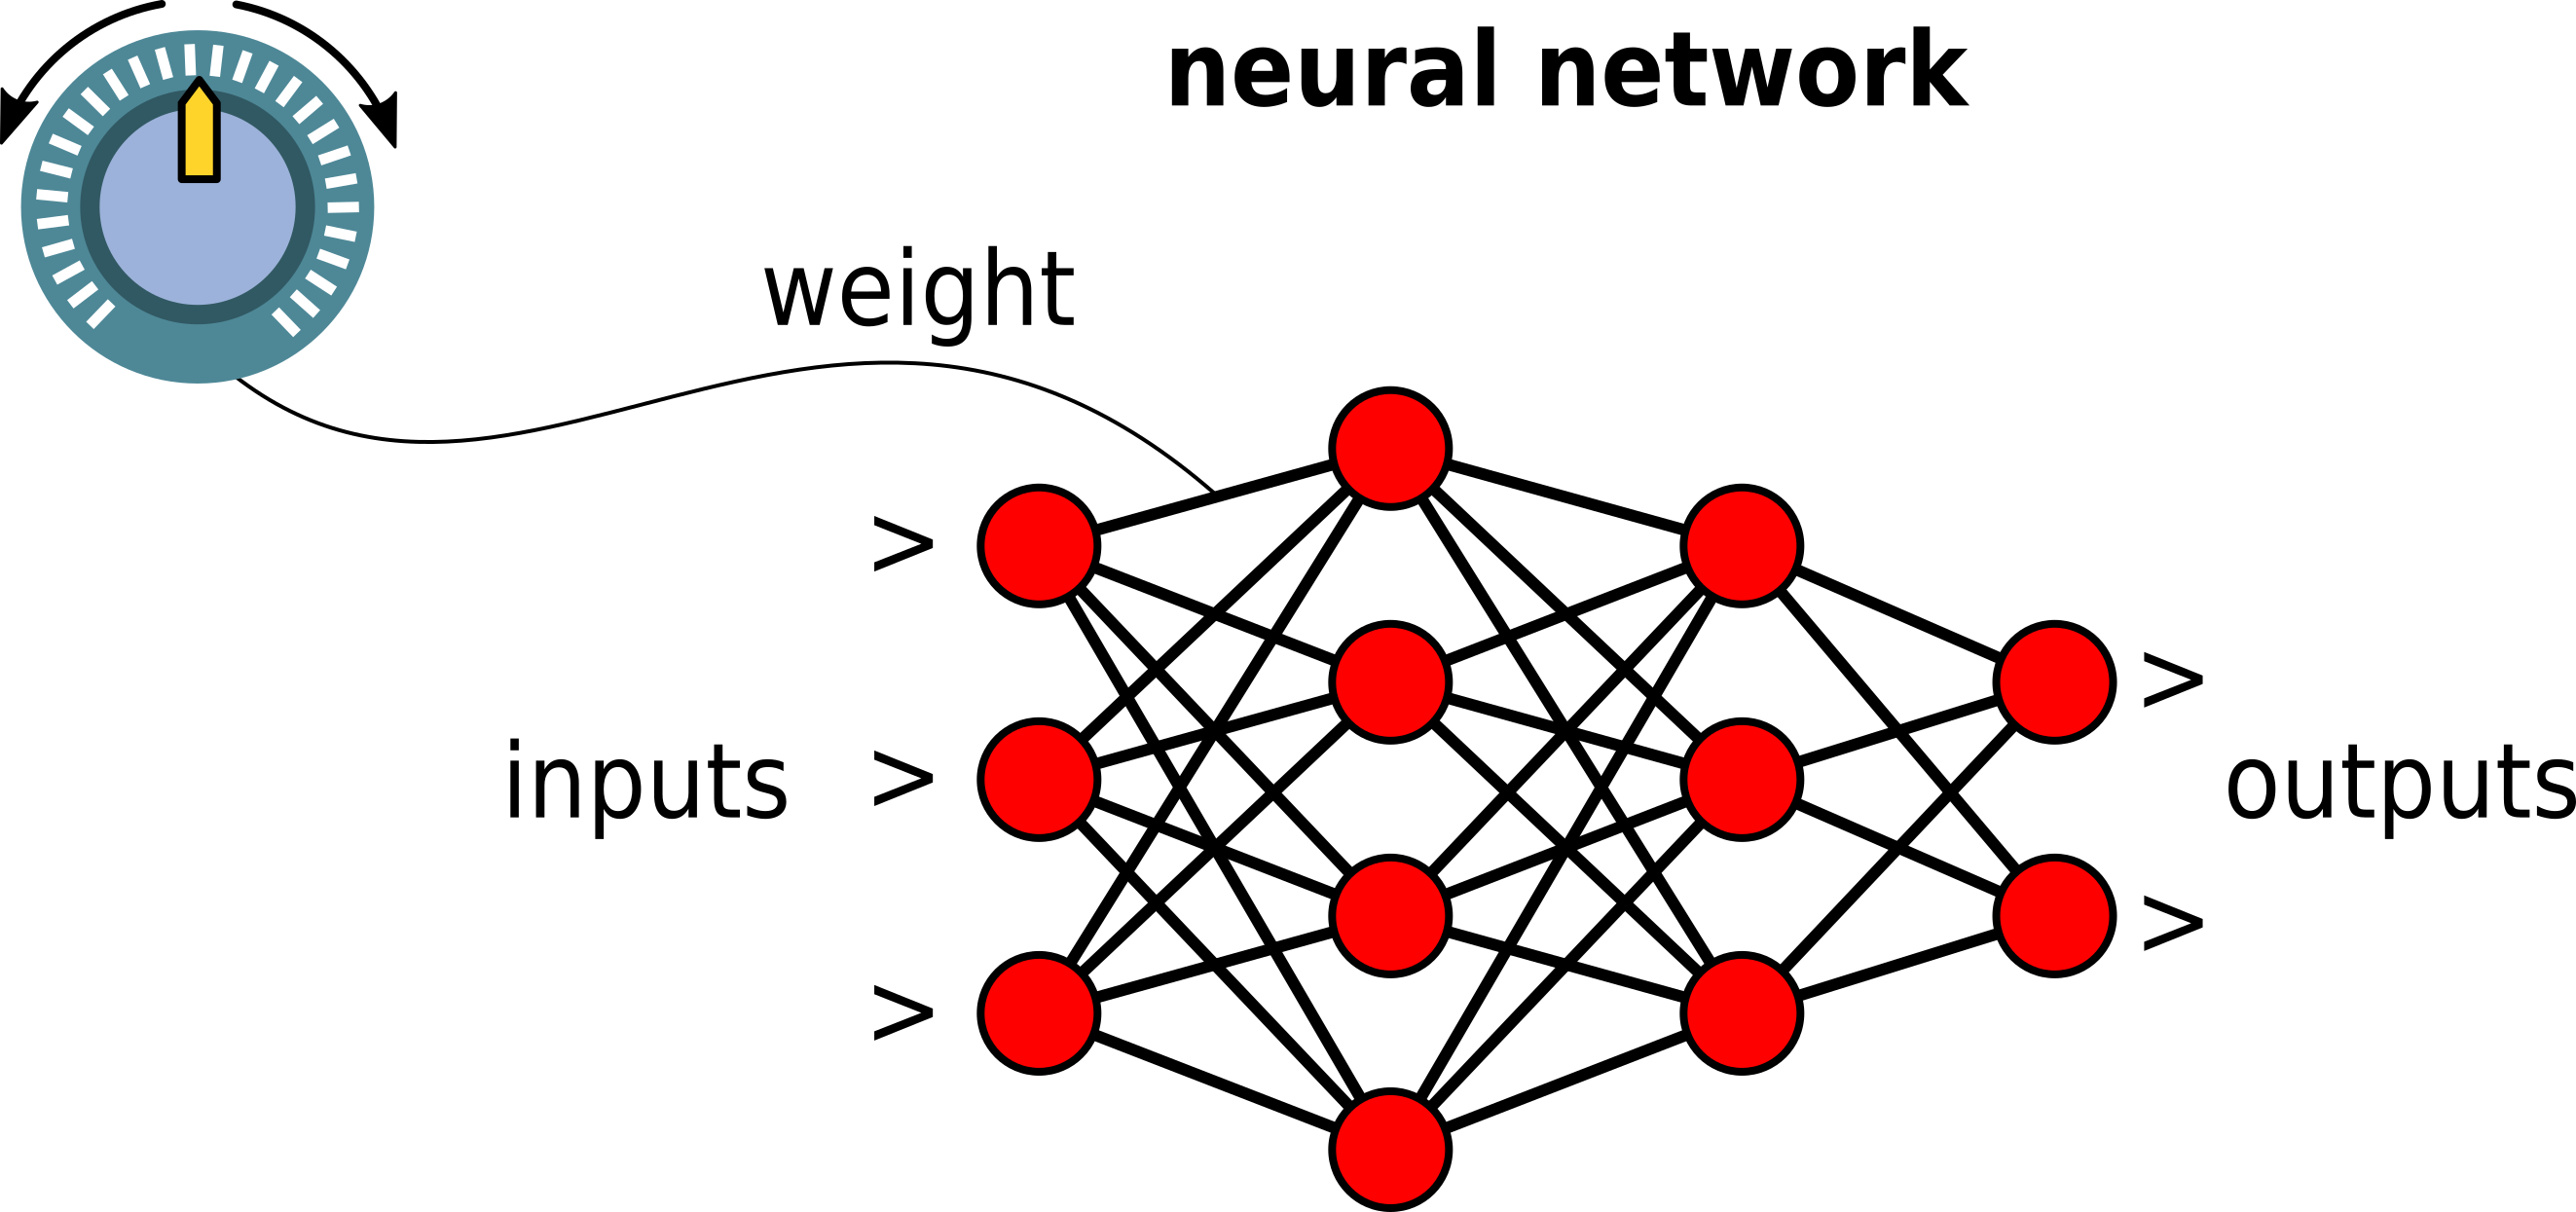
\includegraphics[scale=0.7]{NN-for-dummies.png}}}
\end{equation}

\subsection{Calculus}

\subsection{Vector and matrix}

\end{document}
